\section{Establishing constraints from boundary conditions}
\label{Sec1:estabConstraints}
As the solution is represented as an infinite sum, the coefficients $A_{m,n}^{(i)}$, $B_{m,n}^{(i)}$ and $C_{m,n}^{(i)}$ (coefficients from the fluid domains described below) must be computed for each $n$ (see \Cref{Fig1:coefficients}). By enforcing the boundary conditions in \Cref{Eq1:firstBC,Eq1:secondBC} at each surface, constraints are developed to establish expressions for these coefficients.

\subsection{Notation for the solution in layered domains}
For the $m^{\mathrm{th}}$ solid shell the displacement field from \Cref{Eq1:u_rgen,Eq1:u_tgen} is written as
\begin{equation}
	\vec{u}_m = u_{\mathrm{r},m} \vec{e}_{\mathrm{r}} + u_{\upvartheta,m} \vec{e}_\upvartheta
\end{equation}
where
\begin{align}
	u_{\mathrm{r},m}(r,\vartheta) &= \sum_{n=0}^\infty Q_n^{(0)}(\vartheta)u_{\mathrm{r},m,n}(r) \label{Eq1:u_r}\\
	u_{\upvartheta,m}(r,\vartheta) &= \sum_{n=0}^\infty Q_n^{(1)}(\vartheta)u_{\upvartheta,m,n}(r)
\end{align}
and 
\begin{figure}
	\centering
	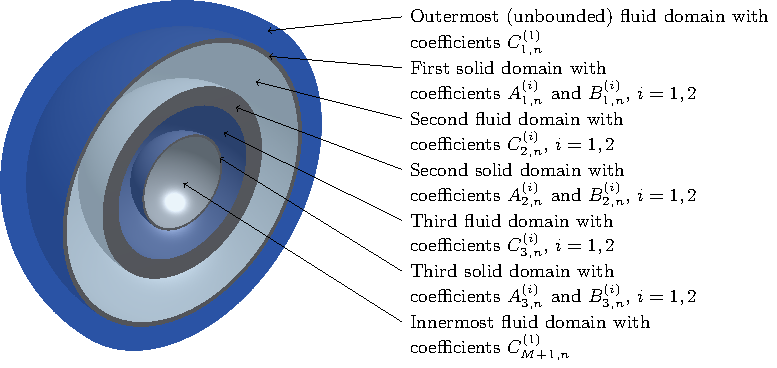
\includegraphics{coefficients_distribution}
	\caption{A model with $M=3$ steel shells with different thicknesses (clip view), illustrating the distribution of the coefficients $A_{m,n}^{(i)}$, $B_{m,n}^{(i)}$ and $C_{m,n}^{(i)}$ over the different domains.}
	\label{Fig1:coefficients}
\end{figure}
\begin{align}
	u_{\mathrm{r},m,n}(r) &= \frac{1}{r}\left[A_{m,n}^{(i)}S_{1,n}^{(i)}(a_m r)+B_{m,n}^{(i)}T_{1,n}^{(i)}(b_m r)\right]\\
	u_{\upvartheta,m,n}(r) &= \frac{1}{r}\left[A_{m,n}^{(i)}S_{2,n}^{(i)}(a_m r)+B_{m,n}^{(i)}T_{2,n}^{(i)}(b_m r)\right].
\end{align}
Corresponding expressions for the stress field in \Cref{Eq1:stress} are obtained as
\begin{align}
	\sigma_{\mathrm{rr},m}(r,\vartheta) &= \sum_{n=0}^\infty Q_n^{(0)}(\vartheta)\sigma_{\mathrm{rr},m,n}(r)\label{Eq1:sigma_rr}\\
	\sigma_{\upvartheta\upvartheta,m}(r,\vartheta) &= \sum_{n=0}^\infty Q_n^{(0)}(\vartheta)\sigma_{\upvartheta\upvartheta,m,n}^{(1)}(r) + Q_n^{(2)}(\vartheta)\sigma_{\upvartheta\upvartheta,m,n}^{(2)}(r)\\
	\sigma_{\upvarphi\upvarphi,m}(r,\vartheta) &= \sum_{n=0}^\infty Q_n^{(0)}(\vartheta)\sigma_{\upvarphi\upvarphi,m,n}^{(1)}(r) +  Q_n^{(1)}(\vartheta)\cot(\vartheta)\sigma_{\upvarphi\upvarphi,m,n}^{(2)}(r)\\
	\sigma_{\mathrm{r}\upvarphi,m}(r,\vartheta) &= 0\\
	\sigma_{\upvartheta\upvarphi,m}(r,\vartheta) &= 0\\
	\sigma_{\mathrm{r}\upvartheta,m}(r,\vartheta) &= \sum_{n=0}^\infty Q_n^{(1)}(\vartheta)\sigma_{\mathrm{r}\upvartheta,m,n}(r)\label{Eq1:sigma_rt}
\end{align}
where
\begin{align*}
	\sigma_{\mathrm{rr},m,n}(r) &= \frac{2G_m}{r^2}\left[A_{m,n}^{(i)} S_{5,n}^{(i)}(a_m r) + B_{m,n}^{(i)} T_{5,n}^{(i)}(b_m r)\right]\\
	\sigma_{\upvartheta\upvartheta,m,n}^{(1)}(r) &= \frac{2G_m}{r^2}\left[A_{m,n}^{(i)} S_{6,n}^{(i)}(a_m r) + B_{m,n}^{(i)} T_{6,n}^{(i)}(b_m r)\right]\\
	\sigma_{\upvartheta\upvartheta,m,n}^{(2)}(r) &= \frac{2G_m}{r^2}\left[A_{m,n}^{(i)} S_{2,n}^{(i)}(a_m r) + B_{m,n}^{(i)} T_{2,n}^{(i)}(b_m r)\right]\\ 
\end{align*}
\begin{align*}
	\sigma_{\upvarphi\upvarphi,m,n}^{(1)}(r) &= \frac{2G_m}{r^2}\left[A_{m,n}^{(i)} S_{6,n}^{(i)}(a_m r) + B_{m,n}^{(i)} T_{6,n}^{(i)}(b_m r)\right]\\
	\sigma_{\upvarphi\upvarphi,m,n}^{(2)}(r) &= \frac{2G_m}{r^2}\left[A_{m,n}^{(i)} S_{2,n}^{(i)}(a_m r) + B_{m,n}^{(i)} T_{2,n}^{(i)}(b_m r)\right]\\ 
	\sigma_{\mathrm{r}\upvartheta,m,n}(r) &= \frac{2G_m}{r^2}\left[A_{m,n}^{(i)} S_{7,n}^{(i)}(a_m r) + B_{m,n}^{(i)} T_{7,n}^{(i)}(b_m r)\right].
\end{align*}

The solution to the Helmholtz equation in the $m^{\mathrm{th}}$ fluid domain (for $2 \leq m \leq M$) has the same general form as $\phi$ in \Cref{Eq1:phiSolutionSimplified}
\begin{equation}\label{Eq1:generalSol}
	p_m(r,\vartheta) = \sum_{n=0}^\infty Q_n^{(0)}(\vartheta)C_{m,n}^{(i)} Z_n^{(i)}(k_m r)
\end{equation}
where the coefficients $C_{m,n}^{(i)}\in\C$ are chosen such that the boundary conditions are satisfied. As the spherical Hankel functions of first and second kind (described in  \Cref{subsec:sphericalBesselAndHankel}) are linear combinations of the spherical Bessel functions of first and second kind, the general solution can be written in terms of these functions. For the outer (unbounded) fluid the Hankel function of the second kind is eliminated due to the Sommerfeld radiation condition in \Cref{Eq1:Sommerfeld}~\cite[p. 26]{Ihlenburg1998fea}. Thus, for the outermost fluid, the scattered pressure field is given by
\begin{equation}\label{Eq1:outerFluid}
	p_1(r,\vartheta) = \sum_{n=0}^\infty Q_n^{(0)}(\vartheta) C_{1,n}^{(1)} \hankel^{(1)}_n(k_1 r).
\end{equation}
Moreover, it is required that the pressure in the innermost fluid domain is\linebreak bounded~\cite[p. 10]{Fender1972sfa}. Hence, the coefficients $C_{M+1,n}^{(2)}$ must be set to zero as the spherical Bessel function of second kind is unbounded at the origin. The pressure in the innermost fluid is therefore given by (cf.~\cite[p. 10]{Fender1972sfa})
\begin{equation}\label{Eq1:innerFluid}
	p_{M+1}(r,\vartheta) = \sum_{n=0}^\infty Q_n^{(0)}(\vartheta) C_{M+1,n}^{(1)} \besselj_n(k_{M+1} r).
\end{equation}
The total pressure in the $m^{\mathrm{th}}$ fluid domain shall be denoted by
\begin{equation}\label{Eq1:totPressure}
	p_{\mathrm{tot},m} =\begin{cases}
	p_1 + p_{\mathrm{inc}}& m = 1\\
	p_m & \text{otherwise}
	\end{cases}	
\end{equation}
where $p_{\mathrm{inc}}$ is the incident wave.

If the coefficients $A_{m,n}^{(i)}$, $B_{m,n}^{(i)}$ and $C_{m,n}^{(i)}$ can be determined, the solution is fully determined in all domains. Hence, a system of equations will be developed to find these coefficients. Indeed, at the boundaries (at a fixed radius) the series can all be written in terms of the Legendre functions $\legendre_n(\cos\vartheta)$, such that the resulting coefficients can be compared for each $n$. A term in the solution is often referred to as a \textit{mode}, such that the resulting constraints from the boundary conditions form a set of \textit{modal equations}. The terminology comes from the vibration analysis~\cite{Chang1994voa}, where each of these modes represent vibration modes. For example, $u_{\mathrm{r},m,n}$ is referred to be the radial displacement in the $m^{\mathrm{th}}$ solid domain in the $n^{\mathrm{th}}$ mode.

\subsection{Tangential traction conditions}
\Cref{Eq1:traction2} is automatically fulfilled due to the axisymmetric assumption. For the $m^{\mathrm{th}}$ shell, evaluating \Cref{Eq1:traction1} at both the inner and outer radius, yields two equations 
\begin{equation}\label{Eq1:tractionCondInserted}
	\sigma_{\mathrm{r}\upvartheta,m,n}(R_{j,m},\vartheta) = 0, \quad j=0,1.
\end{equation}
As $Q_0^{(1)}(\vartheta)=0$, these equations are automatically satisfied for $n=0$. In addition, since $T_{1,0}^{(i)}(\eta)=0$ and $T_{6,0}^{(i)}(\eta)=0$, the coefficients $B_{m,0}^{(i)}$ are redundant (which is convenient, as two constraints are lost in this case). 

Denote by $\vec{H}_{m,n}^{(1)}$, $m=1,\dots,M$, the eigenfrequency matrix\footnote{As illustrated in~\cite{Chang1994voa}, the matrix $\vec{H}_{m,n}^{(1)}$ represent the modal characteristic equations of the $m^{\mathrm{th}}$ shell. That is, the eigenfrequencies of each shell can be found by solving $\det\vec{H}_{m,n}^{(1)}=0$ in terms of the frequency.}~\cite[p. 17]{Chang1994voa} of the $m^{\mathrm{th}}$ shell
\begin{equation}\label{Eq1:K1n}
	\vec{H}_{m,n}^{(1)} = \begin{bmatrix} S_{5,n}^{(1)}(a_m R_{0,m}) & S_{5,n}^{(2)}(a_m R_{0,m}) & T_{5,n}^{(1)}(b_m R_{0,m}) & T_{5,n}^{(2)}(b_m R_{0,m})\\
	S_{7,n}^{(1)}(a_m R_{0,m}) & S_{7,n}^{(2)}(a_m R_{0,m}) & T_{7,n}^{(1)}(b_m R_{0,m}) & T_{7,n}^{(2)}(b_m R_{0,m})\\
	S_{7,n}^{(1)}(a_m R_{1,m}) & S_{7,n}^{(2)}(a_m R_{1,m}) & T_{7,n}^{(1)}(b_m R_{1,m}) & T_{7,n}^{(2)}(b_m R_{1,m})\\
	S_{5,n}^{(1)}(a_m R_{1,m}) & S_{5,n}^{(2)}(a_m R_{1,m}) & T_{5,n}^{(1)}(b_m R_{1,m}) & T_{5,n}^{(2)}(b_m R_{1,m})\end{bmatrix},
\end{equation}
for $n>0$, and 
\begin{equation}\label{Eq1:K10}
	\vec{H}_{m,0}^{(1)} = \begin{bmatrix}	
	 S_{5,0}^{(1)}(a_m R_{0,m}) & S_{5,0}^{(2)}(a_m R_{0,m})\\
	 S_{5,0}^{(1)}(a_m R_{1,m}) & S_{5,0}^{(2)}(a_m R_{1,m})\end{bmatrix},
\end{equation}
for $n=0$. From \Cref{Eq1:sigma_rt,Eq1:sigma_rr} one observes that the first and the last row of $\vec{H}_{m,n}^{(1)}$ correspond to $\sigma_{\mathrm{rr},m,n}(r)$ at $r=R_{0,m}$ and $r=R_{1,m}$, respectively, and the second and third row (for $n>0$) correspond to $\sigma_{\mathrm{r}\upvartheta,m,n}(r)$ at $r=R_{0,m}$ and $r=R_{1,m}$, respectively. The notation $H_{ij,m,n}^{(1)}$, will be used for the elements of the matrices $\vec{H}_{m,n}^{(1)}$.

For $n>0$, the two conditions in \Cref{Eq1:tractionCondInserted} may be written as
\begin{align}
	H_{21,m,n}^{(1)}A_{m,n}^{(1)} + H_{22,m,n}^{(1)}A_{m,n}^{(2)} + H_{23,m,n}^{(1)}B_{m,n}^{(1)} + H_{24,n}^{(1)}B_{m,n}^{(2)} &= 0\\
	H_{31,m,n}^{(1)}A_{m,n}^{(1)} + H_{32,m,n}^{(1)}A_{m,n}^{(2)} + H_{33,m,n}^{(1)}B_{m,n}^{(1)} + H_{34,m,n}^{(1)}B_{m,n}^{(2)} &= 0.
\end{align}
This gives (for each $n$) $2M$ equations in terms of the $6M$ unknown coefficients $A_{m,n}^{(i)}$, $B_{m,n}^{(i)}$ and $C_{m,n}^{(i)}$, $i=1,2$. Thus, an additional $4M$ equations are needed to determine these coefficients. These equations come from the coupling conditions in \Cref{Eq1:firstBC,Eq1:secondBC} (displacement condition and pressure condition, respectively) which are applied at the outer and inner radius of each shell. The outermost and innermost fluid domains will have to be considered separately.

\subsection{Displacement and pressure condition in intermediate fluid layers}
Consider the $m^{\mathrm{th}}$ fluid domain, with $2\leq m\leq M$, where the pressure field is given by \Cref{Eq1:generalSol}. Inserting \Cref{Eq1:u_r,Eq1:generalSol} into the displacement condition in \Cref{Eq1:firstBC} at $r=R_{1,m-1},R_{0,m}$, yields
\begin{align*}
	&\frac{\rho_{\mathrm{f},m}\omega^2}{R_{j,m-j}}\left[A_{m-j,n}^{(i)} S_{1,n}^{(i)}(a_{m-j} R_{j,m-j}) + B_{m-j,n}^{(i)} T_{1,n}^{(i)}(b_{m-j} R_{j,m-j})\right] \\
	&{\hskip12em\relax} - k_m\left[C_{m,n}^{(1)}\besselj_n'(k_m R_{j,m-j}) + C_{m,n}^{(2)}y_n'(k_m R_{j,m-j})\right] = 0
\end{align*}
which yield the relation
\begin{align}
	H_{1,m-j,n}^{(4,j)}A_{m-j,n}^{(1)} + H_{2,m-j,n}^{(4,j)}A_{m-j,n}^{(2)} + H_{3,m-j,n}^{(4,j)}B_{m-1,n}^{(1)} &+ H_{4,m-j,n}^{(4,j)}B_{m-1,n}^{(2)}\nonumber\\ 
	&+ H_{i,m,n}^{(3,j)}C_{m,n}^{(i)} = 0,
\end{align}
for $j=0,1$, where
\begin{align}\label{Eq1:K4}
\begin{split}
	H_{1,m,n}^{(4,j)} &= S_{1,n}^{(1)}(a_m R_{j,m}),\quad H_{2,m,n}^{(4,j)} = S_{1,n}^{(2)}(a_m R_{j,m}),\\ H_{3,m,n}^{(4,j)} &= T_{1,n}^{(1)}(b_m R_{j,m}),\quad H_{4,m,n}^{(4,j)} = T_{1,n}^{(2)}(b_m R_{j,m}),
	\end{split}
\end{align}
and (using \Cref{Eq1:BesselDerivIdentity2} to rewrite the derivative of the Bessel functions)
\begin{align}\label{Eq1:K3}
	H_{i,m,n}^{(3,j)} &= -\frac{1}{\rho_{\mathrm{f},m}\omega^2}\left[nZ_n^{(i)}(\zeta) - \zeta Z_{n+1}^{(i)}(\zeta)\right]\Big\vert_{\zeta=k_mR_{j,m-j}}.
\end{align}

Correspondingly, inserting \Cref{Eq1:sigma_rr,Eq1:innerFluid} into \Cref{Eq1:secondBC} at $r=R_{1,m-1},R_{0,m}$ yields
\begin{align*}
	&\frac{2G_{m-j}}{R_{j,m-j}^2}\left[A_{m-j,n}^{(i)} S_{5,n}^{(i)}(a_{m-j} R_{j,m-j}) + B_{m-j,n}^{(i)} T_{5,n}^{(i)}(b_{m-j} R_{j,m-j})\right] \\
	&{\hskip22em\relax}+ C_{m,n}^{(i)} Z_n^{(i)}(k_m R_{j,m-j}) = 0
\end{align*}
which can be rewritten as
\begin{align}
	H_{11,m-j,n}^{(1)}A_{m-j,n}^{(1)} + H_{12,m-j,n}^{(1)}A_{m-j,n}^{(2)} + H_{13,m-j,n}^{(1)}B_{m-j,n}^{(1)} &+ H_{14,m-j,n}^{(1)}B_{m-j,n}^{(2)}\nonumber\\
	&+ H_{i,m,n}^{(2,j)}C_{m,n}^{(i)} = 0
\end{align}
where
\begin{equation}\label{Eq1:K2}
	H_{i,m,n}^{(2,j)} = \frac{R_{j,m-j}^2}{2G_{m-j}}Z_n^{(i)}(k_mR_{j,m-j}).
\end{equation}


\subsection{Displacement and pressure condition in the outermost fluid}
It is assumed that the incident wave, $p_{\mathrm{inc}}(\vec{x},\omega)$, and its normal derivative at the outermost solid surface can be written on the form
\begin{align}\label{Eq1:IncidentWaveConds}
\begin{split}
	p_{\mathrm{inc}}\Big\vert_{r=R_{0,1}} &= \sum_{n=0}^\infty F_n^{(1)} \legendre_n(\cos\vartheta),\\
	\pderiv{p_{\mathrm{inc}}}{r}\Big\vert_{r=R_{0,1}} &= \sum_{n=0}^\infty F_n^{(2)} \legendre_n(\cos\vartheta),
	\end{split}
\end{align}
respectively. The coefficients $F_n^{(1)}$ and $F_n^{(2)}$ are discussed in \Cref{Sec1:incidentWave}.

Inserting \Cref{Eq1:u_r,Eq1:outerFluid} into the displacement condition in \Cref{Eq1:firstBC} yields
\begin{align*}
	&\frac{\rho_{\mathrm{f},1}\omega^2}{R_{0,1}}\left[A_{n,1}^{(i)} S_{1,n}^{(i)}(a_1 R_{0,1}) + B_{n,1}^{(i)} T_{1,n}^{(i)}(b_1 R_{0,1})\right]  -k_1 C_{1,n}^{(1)} \deriv{\hankel^{(1)}_n}{\zeta}\Big\vert_{\zeta=k_1R_{0,1}} = F_n^{(2)},
\end{align*}
which yields the relation
\begin{equation}
	H_{1,1,n}^{(4,0)}C_{1,n}^{(1)} + H_{2,1,n}^{(4,0)}C_{1,n}^{(2)} + H_{3,1,n}^{(4,0)}C_{1,n}^{(3)} + H_{4,1,n}^{(4,0)}C_{1,n}^{(4)} + H_{1,1,n}^{(3,0)}C_{1,n}^{(1)} = D_{1,n},
\end{equation}
where $H_{i,1,n}^{(4,0)}$ for $i=1,2,3,4$, are given by \Cref{Eq1:K4} and (using \Cref{Eq1:HankelDerivIdentity2})
\begin{equation}\label{Eq1:K3011}
	H_{1,1,n}^{(3,0)} = -\frac{1}{\rho_{\mathrm{f},1}\omega^2}\left[n\hankel^{(1)}_n(\zeta) - \zeta \hankel^{(2)}_{n+1}(\zeta)\right]\Big\vert_{\zeta=k_1R_{0,1}}
\end{equation}
and
\begin{equation}\label{Eq1:D1}
	D_{1,n} = \frac{R_{0,1}}{\rho_{\mathrm{f},1}\omega^2}F_n^{(2)}.
\end{equation}
Correspondingly, by inserting \Cref{Eq1:sigma_rr,Eq1:outerFluid} into \Cref{Eq1:secondBC} one obtains
\begin{align*}
	&\frac{2G_1}{R_{0,1}^2}\left[C_{n,1}^{(1)} S_{5,n}^{(1)}(a_1 R_{0,1}) + C_{n,1}^{(2)} T_{5,n}^{(1)}(b_1 R_{0,1}) + C_{n,1}^{(3)} S_{5,n}^{(2)}(a_1 R_{0,1}) + C_{n,1}^{(4)} T_{5,n}^{(2)}(b_1 R_{0,1})\right] \\
	&{\hskip22.5em\relax} + C_{1,n}^{(1)} \hankel^{(1)}_n(k_1R_{0,1})= -F_n^{(1)},
\end{align*}
which yields the relation
\begin{equation}
	H_{1,1,n}^{(1)}C_{1,n}^{(1)} + H_{2,1,n}^{(1)}C_{1,n}^{(2)} + H_{3,1,n}^{(1)}C_{1,n}^{(3)} + H_{4,1,n}^{(1)}C_{1,n}^{(4)} + H_{1,1,n}^{(2,0)}C_{1,n}^{(1)} = D_{2,n},
\end{equation}
where
\begin{equation}\label{Eq1:K2011}
	H_{1,1,n}^{(2,0)} = \frac{R_{0,1}^2}{2G_1}\hankel^{(1)}_n(k_1R_{0,1})
\end{equation}
and
\begin{equation}\label{Eq1:D2}
	D_{2,n} = -\frac{R_{0,1}^2}{2G_1}F_n^{(1)}.
\end{equation}

\subsection{Displacement and pressure condition in the innermost fluid}
For the innermost fluid the pressure field is given by \Cref{Eq1:innerFluid}. Inserting \Cref{Eq1:u_r,Eq1:innerFluid} into the displacement condition in \Cref{Eq1:firstBC} at $r=R_{1,M}$ yields
\begin{align*}
	&\frac{\rho_{\mathrm{f},M+1}\omega^2}{R_{1,M}}\left[A_{M,n}^{(i)} S_{1,n}^{(i)}(a_M R_{1,M}) + B_{M,n}^{(i)} T_{1,n}^{(i)}(b_M R_{1,M})\right] \\
	&{\hskip16em\relax}- k_{M+1}C_{M+1,n}^{(1)}\besselj_n'(k_{M+1} R_{1,M}) = 0,
\end{align*}
which yields the relation
\begin{equation}
	H_{1,M,n}^{(4,1)}A_{M,n}^{(1)} + H_{2,M,n}^{(4,1)}A_{M,n}^{(2)} + H_{3,M,n}^{(4,1)}B_{M,n}^{(1)} + H_{4,M,n}^{(4,1)}B_{M,n}^{(2)} + H_{1,M+1,n}^{(3,1)}C_{M+1,n}^{(1)} = 0,
\end{equation}
where $H_{i,M,n}^{(4,1)}$ for $i=1,2,3,4$, are defined in \Cref{Eq1:K4}, and 
\begin{equation}\label{Eq1:K311Mp1}
	H_{1,M+1,n}^{(3,1)} = -\frac{1}{\rho_{\mathrm{f},M+1}\omega^2}\left[n\besselj_n(\zeta) - \zeta \besselj_{n+1}(\zeta)\right]\Big\vert_{\zeta=k_{M+1}R_{1,M}}.
\end{equation}
Correspondingly, by inserting \Cref{Eq1:sigma_rr,Eq1:innerFluid} into \Cref{Eq1:secondBC} at $r=R_{1,M}$ the following is obtained
\begin{equation*}
	\frac{2G_M}{R_{1,M}^2}\left[A_{M,n}^{(i)} S_{5,n}^{(i)}(a_M R_{1,M}) + B_{M,n}^{(i)} T_{5,n}^{(i)}(b_M R_{1,M})\right] + C_{M+1,n}^{(1)} \besselj_n(k_{M+1} R_{1,M})  = 0,
\end{equation*}
which yields the relation
\begin{equation}
	H_{11,M,n}^{(1)}A_{M,n}^{(1)} + H_{12,M,n}^{(1)}A_{M,n}^{(2)} + H_{13,M,n}^{(1)}B_{M,n}^{(1)} + H_{14,M,n}^{(1)}B_{M,n}^{(2)}+ H_{1,M+1,n}^{(2,1)}C_{M+1,n}^{(1)} = 0,
\end{equation}
where
\begin{equation}\label{Eq1:K211Mp1}
	H_{1,M+1,n}^{(2,1)} = \frac{R_{1,M}^2}{2G_M}\besselj_n(k_{M+1}R_{1,M}).
\end{equation}


